\chapter{Исследовательская часть}

В этом разделе представлены параметры технического оборудования, на 
котором осуществлялись замеры времени выполнения программного обеспечения, 
а также полученные результаты измерений времени работы.

\section{Постановка цели исследования}

Целью исследования является проведение анализа скорости работы алгоритма генерации одного кадра с помощью алгоритма Z-буфера в 
зависимотси от количества полигонов и шага полигональной сетки.

\section{Технические характеристики}

Технические характеристики устройства, на котором выполнялись замеры времени, представлены далее:

\begin{itemize}
	\item Процессор -- 2 ГЦ 4‑ядерный процессор Intel Core i5;
	\item Оперативная память -- 16 ГБайт;
	\item Операционная система -- macOS Sonoma 14.1.1. 
\end{itemize}

\section{Средство замера времения}

Измерение времени выполнения программы будет проводиться с использованием пакета cgo \cite{cgo}, который внедряет код на языке C~\cite{c}. 
Эта вставка кода будет предназначена для оценки процессорного времени работы программы.

\section{Результаты замера времения}

Для исследования влияния количества полигонов на время генерации изображения проводились замеры, 
в ходе которых размерность сцены изменялась от 10 до 18. Также в процессе исследования происходило изменение шага 
полгональной сетки. Замеры происходили в миллесекундах. Результаты замеров времени приведены в 
таблицы \ref{tb:tbl}. На рисунке \ref{img:graph2} представлена зависимость 
времени выполнения программы от шага полигональной сетки и от размерности сцены.

\begin{table}[!ht]
    \centering
    \caption{\label{tb:tbl}Результаты замера времени (мс)}
    \begin{tabular}{|l|l|l|l|l|l|l|l|l|l|}
        \hline
        \multirow{2}{*}{Шаг полигон. сетки} & \multicolumn{9}{|c|}{Размерность сцены} \\ \cline{2-10}
         & 10 & 11 & 12 & 13 & 14 & 15 & 16 & 17 & 18 \\ \hline
        0.5 & 119 & 172 & 213 & 274 & 322 & 391 & 555 & 916 & 1932 \\ \hline
        0.75 & 125 & 179 & 218 & 283 & 355 & 460 & 569 & 945 & 1994 \\ \hline
        1 & 129 & 182 & 224 & 286 & 363 & 465 & 623 & 1016 & 2098 \\ \hline
        1.25 & 146 & 185 & 229 & 295 & 387 & 485 & 663 & 1039 & 2280 \\ \hline
        1.5 & 148 & 197 & 232 & 321 & 398 & 495 & 743 & 1452 & 2520 \\ \hline
    \end{tabular}
\end{table}

\begin{figure}[h]
    \centering
    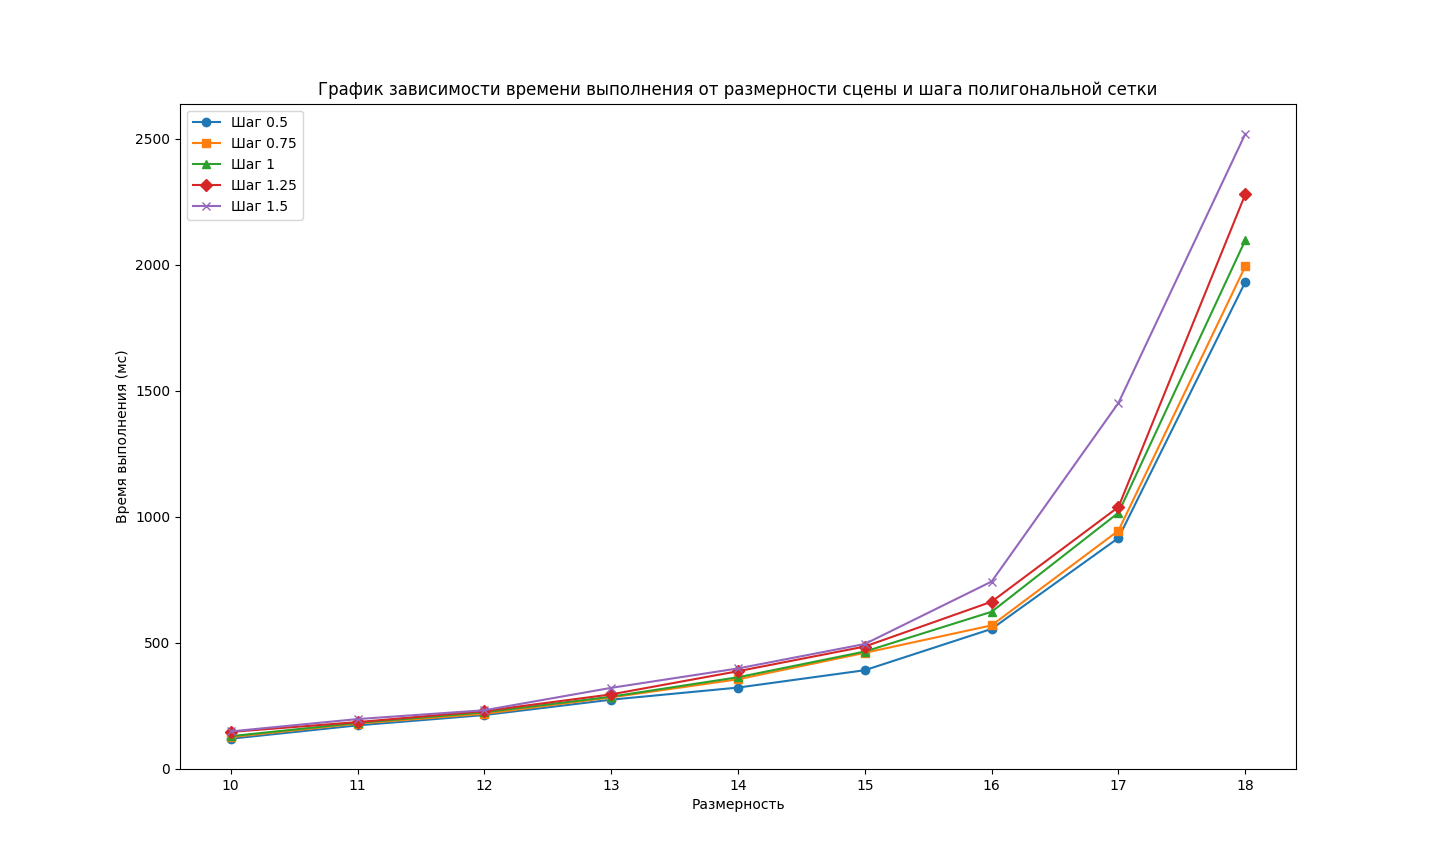
\includegraphics[width=1\linewidth]{img/graph2.png}
    \caption{График зависимости времени генерации одного кадра взависимости от размерности сцены и шага полигональной сетки}
    \label{img:graph2}
\end{figure}
\noindent

\clearpage
На рисунке \ref{img:graph1} представлен приближенный график, иллюстрирующий изменение времени генерации одного кадра 
при размерностях сцены от 10 до 13. Это приближенное представление помогает лучше понять различия в выполнении программы.

\begin{figure}[h]
    \centering
    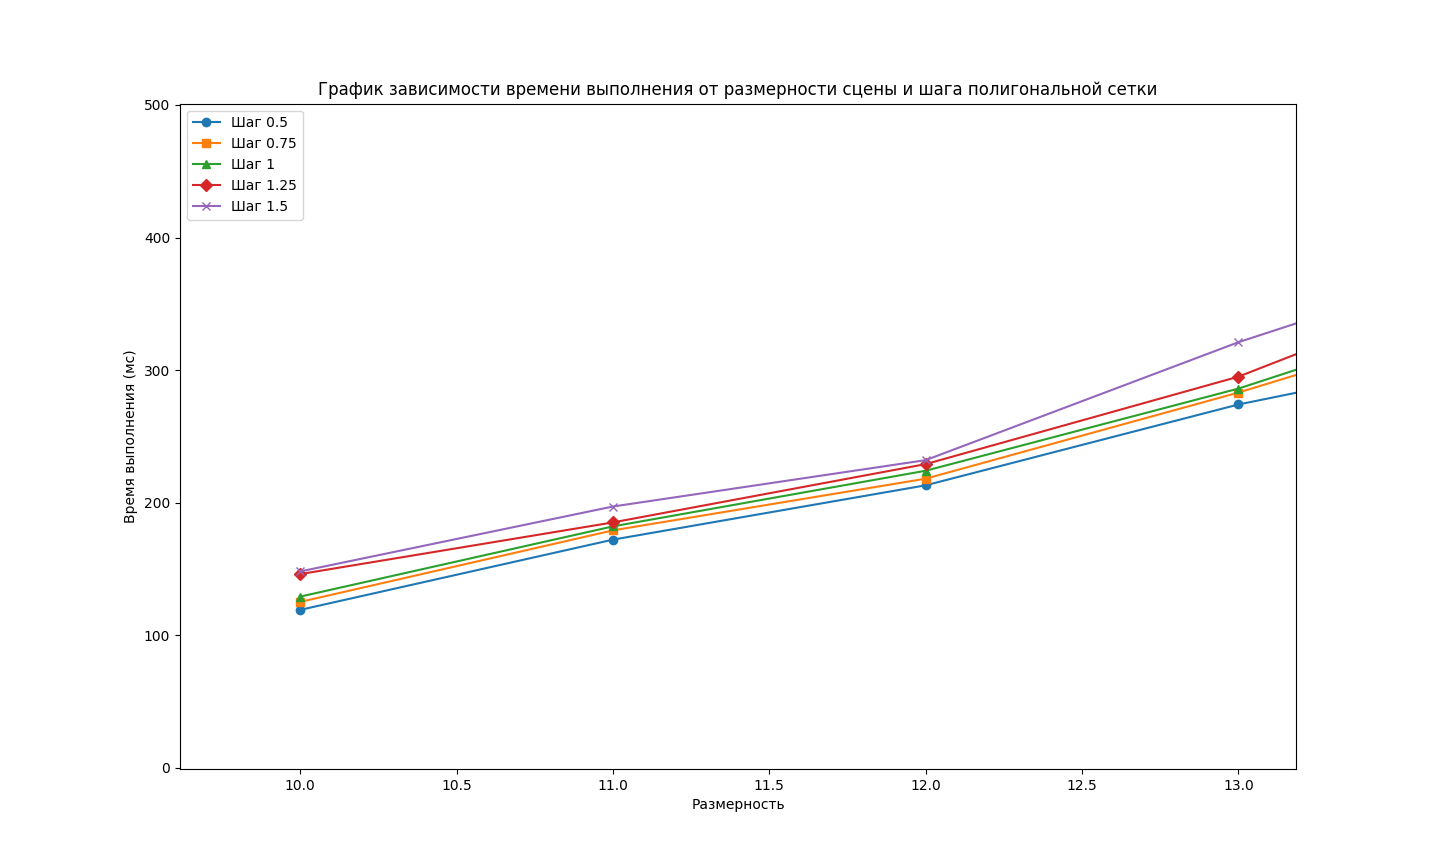
\includegraphics[width=1.1\linewidth]{img/graph1.png}
    \caption{График зависимости времени генерации одного кадра взависимости от размерности сцены и шага полигональной сетки}
    \label{img:graph1}
\end{figure}
\noindent
